\subsection{Ambiguities}
\label{sec:parsing-ambiguities}

When a sentence contains a lexical entry that corresponds to multiple elementary LTAG/DUDES in grammar, we say that an \textit{ambiguity} is occurring.
%
A \textit{syntactic ambiguity} occurs when an entry corresponds to multiple elementary LTAG/DUDES with different LTAG
%
A \textit{semantic ambiguity} occures when and entry corresponds to multiple elementary LTAG/DUDES, with same LTAG and different DUDES.
%
Typically, a syntactic ambiguity is easier to solve than a semantic one, because the former can be solved by structural analysis of LTAG, while the latter needs some resoning steps.

In our solution, we solve both form of ambiguities.
%
In particular, when ambiguities arise, the colliding LTAG are structurally analyzed to filter out all syntactic ambiguities.
%
All semantic ambiguities are solved by checking the consistency of their DUDES with respect to the given ontology.

In Figure~\ref{fig:ambiguities-1} and Figure~\ref{fig:ambiguities-2} we give an example of ambiguities resolution.
%
Let us consider the question \textit{'Is Satya Nadella italian?'}. Here we have the following ambiguities:

\begin{itemize}
\item the entry \textit{'is'} induces a syntactic ambiguity because it corresponds to the elementary LTAG/DUDES with LTAG (a) and (b).
%
The ambiguity is solved by excluding (a), because it contains a substitution node on the left of the lexical entry, hence it cannot suitable to parse the first word of a sentence. 
%
Finally, (b) is considered as to be the only feasible LTAG/DUDES.

\item the entry \textit{'italian'} induces a syntactic/semantic ambiguity because it corresponds to the elementary LTAG/DUDES with LTAG (c)/(d) and DUDES (e)/(f).
%
The ambiguity is solved in two steps.
%
First, the LTAGs (d) with DUDES (e) and (f) are excluded because they cannot be adjuncted to the main LTAG/DUDES.
%
Then, (f) is excluded because the proposition \textit{hasHeadquarter(x,y)} cannot have domain \textit{Person} as the entry `Satya Nadella` has.
%
Finally, the LTAG (c) with DUDES (e) is considered as to be the only feasible LTAG/DUDES.
\end{itemize}

\begin{figure}[tp]
\caption{An example of syntactic ambiguity resolution. Ambiguous LTAG for the entry \textit{'is'}.}
\label{fig:ambiguities-1}
	\begin{tabular}{ p{10em} p{10em} }
		\begin{center}
			(a)
			\begin{tikzpicture}
			\Tree [.S [.DP$_1\downarrow$ ] [.VP [.V is ] [.DP$_2\downarrow$ ] ] ]
			\end{tikzpicture}
		\end{center}		
		&
		\begin{center}
			(b)
			\begin{tikzpicture}
			\Tree [.S [.VP [.V is ] [.DP$_1\downarrow$ ] ] [.DP$_2\downarrow$ ] ]
			\end{tikzpicture}
		\end{center}
	\end{tabular}
\end{figure}

\begin{figure}[tp]
\caption{An example of syntactic/semantic ambiguity resolution. Ambiguous LTAG/DUDES for the entry \textit{'italian'}.}
\label{fig:ambiguities-2}
\begin{tabular}{ p{10em} p{10em} }
	\begin{center}
	(c)
	\begin{tikzpicture}
	\Tree [.DP [.ADJ italian ] ]
	\end{tikzpicture}
	\end{center}		
	&
	\begin{center}
	(d)
	\begin{tikzpicture}
	\Tree [.NP [.ADJ italian ] [.NP* ] ]
	\end{tikzpicture}
	\end{center}		
	\\
	\begin{center}
	(e)
	\begin{tabular}{|c|l|}
		\hline
		\mbox{x} & \\ 
		\hline
		\multicolumn{2}{|l|}{
			$hasNationality(x,y)$
		}\\
		\multicolumn{2}{|l|}{
			$y=Italy$
		}\\
		\hline
		\multicolumn{2}{|l|}{
			\mbox{}
		}\\
		\hline
	\end{tabular}
	\end{center}
	&
	\begin{center}
	(f)
	\begin{tabular}{|c|l|}
		\hline
		\mbox{x} & \\ 
		\hline
		\multicolumn{2}{|l|}{
			$hasHeadquarter(x,y)$
		}\\
		\multicolumn{2}{|l|}{
			$y=Italy$
		}\\
		\hline
		\multicolumn{2}{|l|}{
			\mbox{}
		}\\
		\hline
	\end{tabular}
	\end{center}	
\end{tabular}
\end{figure}

Our parse leverages a reasoning step to solve semantic ambiguities.
%
Whenever a semantic ambiguities arise, a SPARQL query is generated from the DRS statements of each ambiguous DUDES to test its feasibility.

In the following Figures~\ref{fig:ambiguities-resolution-a}-\ref{fig:ambiguities-sparql} we can see an example.
%
Let us consider the main LTAG/DUDES (a) and the ambiguous LTAG/DUDES.
%
The feasibility of DUDES in (b) with respect to (a) is tested by the SPARQL query in Figure~\ref{fig:ambiguities-sparql}. Since the query returns True only for the second DUDES, the first one is excluded.

\begin{figure}[tp]
\caption{An example of ambiguity resolution through reasoning. The main LTAG/DUDES (a)}
\label{fig:ambiguities-resolution-a}
\begin{tabular}{ p{10em} p{10em} }
	\begin{center}
	\begin{tikzpicture}
	\Tree [.S [.VP [.V is ] [.DP$_1$ Microsoft ] ] [.DP$_2\downarrow$ ] ]
	\end{tikzpicture}
	\end{center}		
	&
	\begin{center}
	\begin{tabular}{|c|l|}
		\hline
		\mbox{} & x y \\ 
		\hline
		\multicolumn{2}{|l|}{
			$x=Microsoft$
		}\\
		\multicolumn{2}{|l|}{
			$x=y$
		}\\
		\hline
		\multicolumn{2}{|l|}{
			\mbox{$(y,DP_2)$}
		}\\
		\hline
	\end{tabular}
	\end{center}
\end{tabular}
\end{figure}

\begin{figure}[tp]
\caption{An example of ambiguity resolution through reasoning. The LTAG/DUDES that must be checked for semantic feasibility (b)}
\label{fig:ambiguities-resolution-b}
\begin{tabular}{ p{10em} p{10em} p{10em} }
	\begin{center}
	\begin{tikzpicture}
	\Tree [.DP [.ADJ italian ] ]	
	\end{tikzpicture}
	\end{center}		
	&
	\begin{center}
	\begin{tabular}{|c|l|}
		\hline
		\mbox{x} & x y \\ 
		\hline
		\multicolumn{2}{|l|}{
			$hasNationality(x,y)$
		}\\
		\multicolumn{2}{|l|}{
			$y=Italy$
		}\\
		\hline
		\multicolumn{2}{|l|}{
			\mbox{}
		} \\
		\hline
	\end{tabular}
	\end{center}
	&
	\begin{center}
	\begin{tabular}{|c|l|}
		\hline
		\mbox{x} & x y \\ 
		\hline
		\multicolumn{2}{|l|}{
			$hasHeadquarter(x,y)$
		}\\
		\multicolumn{2}{|l|}{
			$y=Italy$
		}\\
		\hline
		\multicolumn{2}{|l|}{
			\mbox{}
		} \\
		\hline
	\end{tabular}
	\end{center}	
\end{tabular}
\end{figure}

\begin{figure}[tp]
\caption{An example of ambiguity resolution though reasoning. The SPARQL query to test semantic feasibility for ambiguity in Figure~\ref{fig:ambiguities-resolution-b}.}
\label{fig:ambiguities-sparql}
\begin{center}
\begin{verbatim}
ASK WHERE {
    :Microsoft rdf:type ?class1 . 
    :Italy rdf:type ?class2 . 
    hasNationality rdfs:domain ?class1 . 
    hasNationality rdfs:range ?class2
} 
\end{verbatim}	
\end{center}
\end{figure}